% \glsresetall
\chapter{Webpack Module Federation} % Main chapter title
\label{Chapter5}

\lhead{Chapter 5. \emph{Webpack Module Federation}}

Since an introduction of this technology was given in chapter \ref{Chapter2}, only a short recap of WMF is given here. Main focus of this chapter will be, to showcase how the technology was implemented in the prototype. As mentioned before, the implementation of the WMF was mainly done in combination with Angular. Therefore, all the examples and explanations below will have a focus on exactly that framework. It has to be mentioned though, that WMF is not restricted on Angular alone. The only restriction applied is concerning the bundler, which has to be Webpack.\cite{wmf_concepts}

\section{Short recap}

WMF is a new way to create micro frontends using the Webpack bundler in version 5. The way it does that is via modularization of self-compiled code parts and publish them for integration by other modules. This published modules can be micro frontends them selfs and are called remotes whereas the integrating modules are called hosts. 
Hosts refer to remotes under a configured name, this name is not actually known to the host during the compile time, but is first resolved at runtime.
The self compiled remote in this case can be anything, a micro frontend or some sort script for utility. This way the Module Federation provides a way to avoid external or manual script loading and instead gives opportunities to automatically lazy load necessary code blocks during runtime.\cite{wmf_concepts}

Integration several remotes using the same dependencies leads to redundancies and for that WMF offers a solution as well. Via configuration of shared dependencies WMF provides a way to reduce redundant libraries in its landscape. A more detailed explanation was given in \ref{Chapter2}.

\section{Implementation in the prototype}

As previously mentioned the main functionality of WMF used in the prototype, is sharing of dependency feature. Below it is explained how it was implemented and an overview of the landscape is given.

For the WMF landscape of the prototype the Angular framework was used. To component library for the user interface was \texttt{@Fundamental-NGX/Core}. To showcase the handling of shared libraries and multi versions in a micro frontend landscape with WMF, several WMF project where created and accordingly configured.
For the rest of this chapter the WMF specific terminology will be used.

\begin{itemize}
	\item \textbf{Same versions} - This is the host containing remotes of the same Angular version. The dependency itself is shared. This application was implemented to use it as comparison to the multi version hosts.
	
	\item \textbf{Mixed versions} - This is the host contains partially the same and different Angular versions. Each version of the library is shared inside the landscape between the remotes. Purpose of this implementation was to showcase how many redundant versions of the same library are maintained by WMF in a multi version landscape and how its affects the performance.
	
	\item \textbf{Different versions} - This host contains only different Angular versions. Therefore, it is an extreme version of the \textit{Mixed versions} implementation. Every remote published, requires a different version of Angular. Goal with this implementation was to showcase the performance losses in a so called in comparison to the other two landscapes. It rather serves as a negative example of how WMF should not be used.
\end{itemize}

To guarantee a basis for comparison, the user interface of each remote is the same. The figure below shows the elements displayed in each remote.

\begin{figure}[!h]
	\centering
	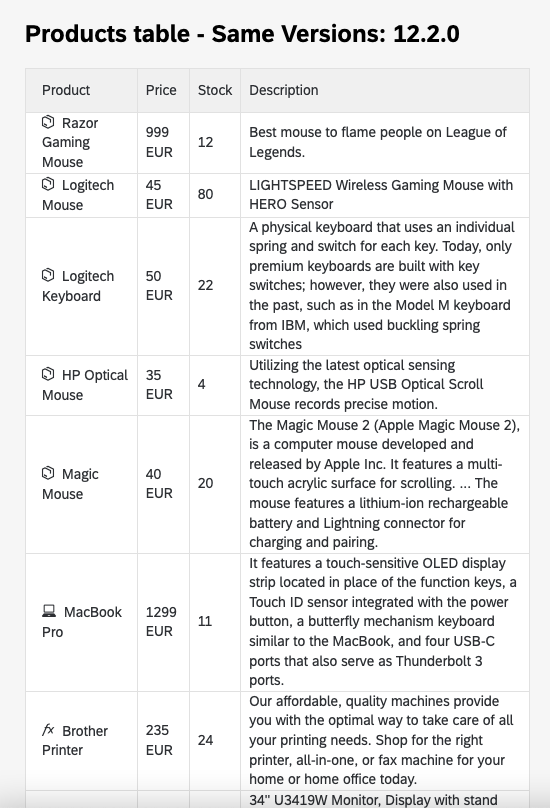
\includegraphics[width=0.7\textwidth]{Figures/WMF_SameVersions.png}
	\caption{Example of an implemented remote in the prototype WMF landscape}
	\label{fig:wmf_screenshot}
\end{figure}

Figure \ref{fig:wmf_screenshot} shows the elements of a remote in the WMF prototype. It contains a table with several table items in it. The angular version of each element is displayed above in the header.

 \subsection{The Webpack bundler}
 
Prior to introducing the implemented landscape in detail, it is necessary to talk about Webpack itself first. As mentioned before, Webpack a mandatory feature for using the Module Federation. Popular UI frameworks like React, VueJS or Angular use Webpack under the hood anyway, it isn't as much of a restriction as it seems.\cite{webpack_angular}\cite{webpack_react}\cite{webpack_vue}
The documentation of the named frameworks, imply that Webpack is used by default, but can be customized if necessary by the developer.

For Angular in particular, it is necessary to install two dependencies via the Angular CLI, to enable the features of the Module Federation. The command sused for this is the following. 

\begin{lstlisting}[language=Bash, caption=Angular CLI console command to enable Module Federation in an Angular project, label=angluar_wmf_command]
ng add @angular-architects/module-federation --project name --port port
\end{lstlisting}

These commands enable the Module Federation for an Angular project. Since the CLI protects the Webpack configuration from access, a custom builder is required. The \texttt{@angular-architects/module-federation} package provides exactly that.
After installing this dependency in an Angular project, a \texttt{webpack.config.js} will appear on root level of the corresponding project.\cite{wmf_angular_dependency_install}
This dependency has to be added in each remote or host of the WMF landscape. Since every component is handled as a separate project.

After enabling the Module Federation inside a project, the necessary configuration can be applied to the \texttt{webpack.config.js} file. The remotes publish their modules and hosts consume them. Thus a developer can distinguish what module has which role.
The examples of such configurations for hosts and remotes are shown below in the section accompanied by the usage if the shared dependency features.

Since the implementation of the remotes is always similar, it wont be mentioned. Instead the configurations of the corresponding \texttt{webpack.config.js} files will be explained in addition to the project structures.

\subsection{Implementation of the prototype versions}

The three implemented versions for the the WMF landscape are fairly similar to each other, the only difference can be found the dependencies and the configured sharing. Below a listing of the configuration for the \textit{sameVersion} environment can be found.

\begin{lstlisting}[language=JavaScript, caption=Content of \texttt{webpack.config.js} of the shell of the same versions WMF project, label=wmf_sameversions_shell]
[...]
module.exports = {
	[...]
	plugins: [
	new ModuleFederationPlugin({
		name: "shell",
		filename: "remoteEntry.js",
		shared: share({
			"@angular/core": { 
				singleton: true, 
				strictVersion: false, 
				requiredVersion: '= 12.2.0'
			},
			"@angular/common": { 
				singleton: true, 
				strictVersion: false, 
				requiredVersion: '= 12.2.0' 
			},
			...sharedMappings.getDescriptors()
		})
		
	}),
	sharedMappings.getPlugin()
	]};
\end{lstlisting}

Listing \ref{wmf_sameversions_shell} shows the configuration of the shell/host application. As it can be seen the shared dependencies are defined in between lines 22 and 24. Line 18 and 19 define the name of the application in the landscape and the name of the file after bundling. For the above case it has to be mentioned that the remotes are separate applications in their own runtime. Therefore, they have to be imported via the network. Thus no \texttt{remote} property is configured in this file. To add the dynamically loaded remotes, a service had to be developed which imports the remotes at runtime. This service is shown in below listing.\cite{wmf_angular_dynamicfederation}

\begin{lstlisting}[language=JavaScript, caption=Content of \texttt{lookup.service.ts} for remote module loading in shell applications, label=wmf_lookup_service]
[...]
@Injectable({ providedIn: 'root' })
export class LookupService {
	lookup(): Promise<PluginOptions[]> {
		return Promise.resolve([
		{
			remoteEntry: 'https://angular-wmf-same-mfe1.surge.sh/remoteEntry.js',
			remoteName: 'mfe1',
			exposedModule: './Mfe1',
			
			displayName: 'Mfe1',
			componentName: 'Mfe1Component'
		},
		[...]	
		] as PluginOptions[]);
	}
}
\end{lstlisting}

This service serves the information of the remotely loaded modules to plugins for actual rendering. The rendering itself is done in a proxy plugin component. This component defines a plain template as a some sort of placeholder for the remotes. \cite{wmf_angular_dynamicfederation}
\newpage
\begin{lstlisting}[language=JavaScript, caption=Content of \texttt{plugin-proxy.component.ts} for remote module loading in shell applications, label=wmf_pluginproxy]
[...]	
@Component({
	selector: 'plugin-proxy',
	template: `
	<ng-container #placeHolder></ng-container>
	`
})
export class PluginProxyComponent implements OnChanges {
	@ViewChild('placeHolder', { read: ViewContainerRef, static: true })
	viewContainer: ViewContainerRef;
	
	constructor(
		private injector: Injector,
		private cfr: ComponentFactoryResolver) { }
	
	@Input() options: PluginOptions;
	
	async ngOnChanges() {
		this.viewContainer.clear();
		
		const Component = await loadRemoteModule(this.options)
		.then(m => m[this.options.componentName]);
		
		const factory = this.cfr.resolveComponentFactory(Component);
		const compRef = this.viewContainer.createComponent(factory, null, this.injector);		
	}
}
\end{lstlisting}

Line 8 of listing \ref{wmf_pluginproxy} defines the \texttt{ng-container} with the identifier called \texttt{placeholder}. This identifier is used in the code below to select and actually fill the container with a remote module. The functionality is placed in one of Angulars Lifecycle hook methods \texttt{ngOnChanges}, which is triggered when changes to input proprieties occur.\cite{wmf_angular_lifecyclehooks} 
In there the container is first cleared, then a remote loading option is selected from the array of the \texttt{lookup.service.ts}. The following line, create an Angular component out of the loaded remote and insert it into the placeholder container, using the imported dependencies.
The type of the plugin options was defined in an interface, exporting a type definition. The code for it can be found below.
\newpage
\begin{lstlisting}[language=JavaScript, caption=Content of \texttt{plugin.ts} for remote module loading in shell applications, label=wmf_plugintype]
import { LoadRemoteModuleOptions } from '@angular-architects/module-federation';
export type PluginOptions = LoadRemoteModuleOptions & {
	displayName: string;
	componentName: string;
};
\end{lstlisting}

The previously imported \texttt{@angular-architects/module-federation} dependency offers an existing type interface for that use case. This is extended by two more properties in line 4 and 5 of listing \ref{wmf_plugintype}.
By configuring the above service and component, it is made possible to load federated modules via the network into the host application.
The configuration for a federated module can be seen below.

\begin{lstlisting}[language=JavaScript, caption=Content of \texttt{webpack.config.js} of the mfe1 remote app of the same versions WMF project, label=wmf_sameversions_mfe1]
[...]
module.exports = {
	[...]
	plugins: [
	new ModuleFederationPlugin({
		name: "mfe1",
		filename: "remoteEntry.js",
		exposes: {
			'./Mfe1': './src/app/mfe1.component.ts'
		},
		shared: share({
			"@angular/core": { 
				singleton: true, 
				strictVersion: false, 
				requiredVersion: '<= 12.2.0' 
			},
			"@angular/common": { 
				singleton: true, 
				strictVersion: false, 
				requiredVersion: '<= 12.2.0' 
			},
			"@fundamental-ngx/core": { 
				singleton: true, 
				strictVersion: false,
				requiredVersion: '0.33.0-rc.214' 
			},
			...sharedMappings.getDescriptors()
		})
	}),
	sharedMappings.getPlugin()
	]};
\end{lstlisting}

As mentioned in chapter \ref{Chapter2} every remote participating at sharing dependencies has to bulk in. Therefore, a similar sharing configuration as the is one of the the shell can be found in the remotes. 
Between line 7 and 11, the actual federation of the module is configured. The reference to the module is later bundles in a file with the name defined in the \texttt{filename} property. In this case it is the \texttt{remoteEntry.js}.
This is the file is automatically generated when the remote is compiled and serves as the entry point for the application when it is loaded into the host. Therefore this is the file accessed via the server url in the \texttt{lookup.service.ts} \ref{wmf_lookup_service}.
As soon as the script is loaded via the service, the exposed module paths and names become known to the host and can be used to load the module. Thus the \texttt{expose} property contains a Java Script object, which maps the path to the actual component to \texttt{./Mfe1} in this case.\cite{wmf_concepts}

The implementations of the versions is similar and differs in the the shared dependencies configured. The effects of a multi version environment and how it is handled by the Module Federation were explained in chapter \ref{Chapter2}.